\documentclass[class=article,border=5pt,tikz]{standalone}
\usetikzlibrary{shapes.geometric}

\tikzset{myhex/.style={regular polygon,regular polygon sides=6,draw,
    outer sep=0pt,minimum width=3cm,
    append after command={[/utils/exec=\let\mylastnode\tikzlastnode]
foreach \x  in {1,...,6} {(\mylastnode.corner \x)
node[draw,shape=circle,fill=white,minimum size=6mm]{}}
}}}%

\begin{document}
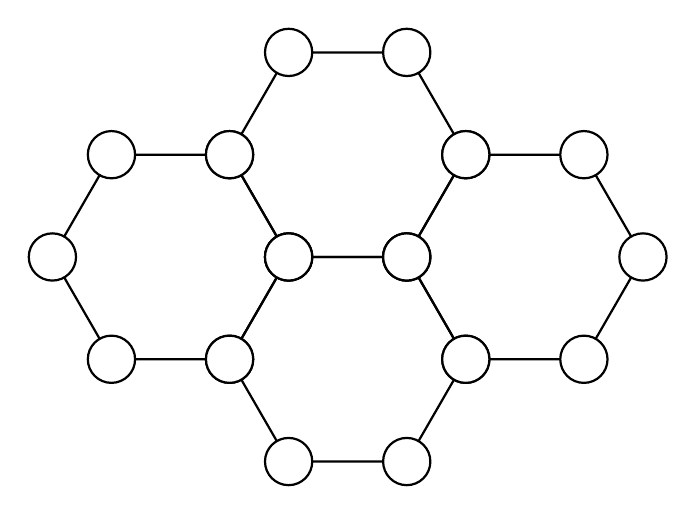
\begin{tikzpicture}[thick,x=1cm,y=1cm]
  \path (0,0) node[myhex] (h1) {}
    node[myhex,anchor=corner 3]  (h2) at (h1.corner 1){}
    node[myhex,anchor=corner 3]  (h3) at (h1.corner 5){}
    node[myhex,anchor=corner 3]  (h4) at (h2.corner 5){};
\end{tikzpicture}
\end{document}